\section{\sysname design}
\label{sec:system-design}

\sysname is designed to impose minimal burden on authors. The benefit of automatic consistency between the experiments and the text should provide more than sufficient incentive for the minor effort required to use \sysname.

%%%%%%%%%%%%%%%%%%%%%%%%%%%%%%%%%%%%%%%%%%%%%%%%%%%%%%
%%%%%%%%%%%%%%%%%%%%%%%%%%%%%%%%%%%%%%%%%%%%%%%%%%%%%%
%%%%%%%%%%%%%%%%%%%%%%%%%%%%%%%%%%%%%%%%%%%%%%%%%%%%%%
%%%%%%%%%%%%%%%%%%%%%%%%%%%%%%%%%%%%%%%%%%%%%%%%%%%%%%
%%%%%%%%%%%%%%%%%%%%%%%%%%%%%%%%%%%%%%%%%%%%%%%%%%%%%%

\subsection{Overview}
\label{sec:workflow}

At a high level, \sysname augments \LaTeX{} with a markup language to: (a) capture inputs to the experiments; and (b) create placeholders for text and plots showing results. When the marked-up \LaTeX{} source is compiled, \sysname parses the inputs and invokes the authors' experiment code. For creating the final PDF, the generated results are used to replace placeholders in the text.
End-to-end, the following steps, as illustrated in Fig.~\ref{fig:architecture}, create a \sysname-enabled paper:


\begin{itemize}[leftmargin=12pt,itemsep=2pt,topsep=2pt]
    \item The authors use a lightweight markup language to annotate inputs, parameters, configurations, etc. in their \LaTeX{} source. They also annotate placeholders for text about results, as well as result plots.
    \item \sysname interprets the markup throughout the paper in a single pass, and creates input files for the authors' experiment framework(s). Each experiment is executed with its specified inputs to generate the outputs.
    \item \sysname invokes the authors' post-processing routine(s) to generate any plots and result metric values with the labels matching the corresponding placeholders.
    \item The last step is a traditional \LaTeX{} compilation, not specific to \sysname, to create the document.
\end{itemize}

\noindent A key design choice is to not overly restrict how experiments are specified, \eg with a limited domain-specific language. Instead, given the diversity of experimental methods and frameworks, \sysname relies on general purpose hooks to invoke the authors' experiment framework(s) with appropriate input and output files. The authors themselves decide what constitutes an experiment, and how it can be modified, parameterized, analyzed, and presented. The authors use the markup to express these decisions, and provide means to invoke their experiment framework(s) with the input files \sysname creates from parsing the markup. The experiment framework can be \emph{anything} that: (a) accepts input files and outputs result / log files; and (b) can be executed by others without depending on custom hardware, bespoke testbeds, etc.

Today's typical workflow involves experiment run scripts in authors' code, which the authors execute, and manually extract the resulting data and plots from, to add to their paper's text. In contrast, \sysname makes the paper's text itself the collection of ``run scripts'', using them to control the experiments, and to automatically ingest the resulting outputs.

% Architecture overview
\begin{figure}
 \begin{center}
  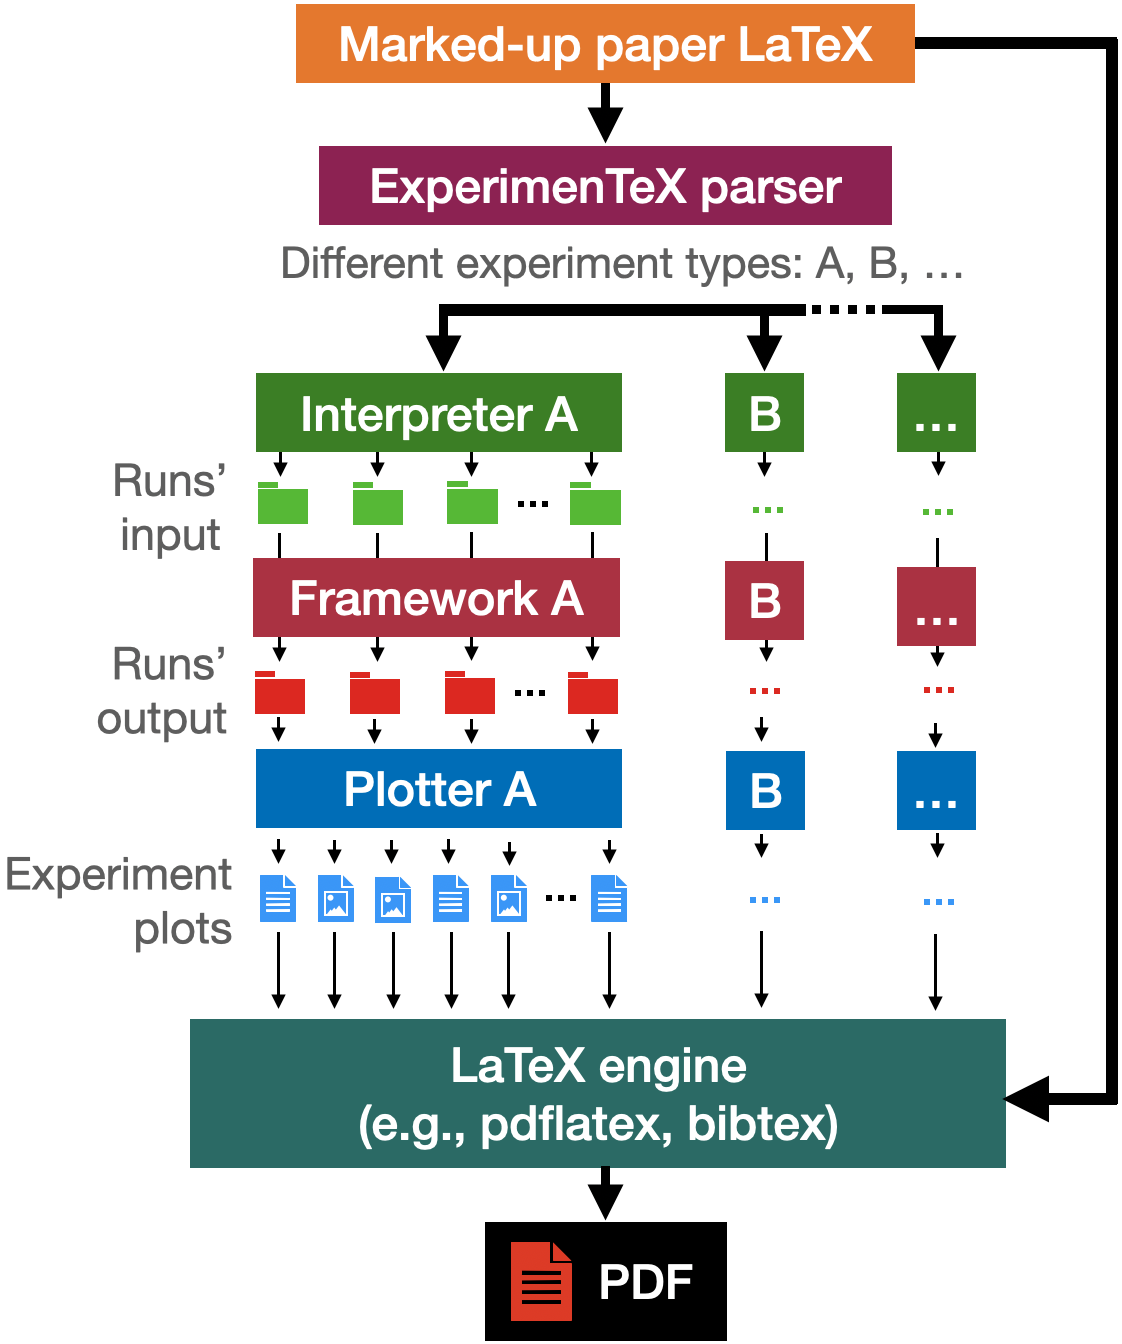
\includegraphics[width=0.47\textwidth]{figures/architecture.png}
  \caption{\sysname overview: authors use simple markup in \LaTeX{}, which our parser parses. Authors' code itself must translate the parsed representations to create inputs for the authors' experiment framework(s), and to identify the result text and plots needed. The experiments are invoked on the inputs, and the authors' post-processing and plotting pipelines are used to generate the result text and plots. A standard \LaTeX{} compile uses these resources to create the PDF.}
  \vspace{-5pt}
  \label{fig:architecture}
  \vspace{0pt}
 \end{center}
\end{figure}

%%%%%%%%%%%%%%%%%%%%%%%%%%%%%%%%%%%%%%%%%%%%%%%%%%%%%%
%%%%%%%%%%%%%%%%%%%%%%%%%%%%%%%%%%%%%%%%%%%%%%%%%%%%%%
%%%%%%%%%%%%%%%%%%%%%%%%%%%%%%%%%%%%%%%%%%%%%%%%%%%%%%
%%%%%%%%%%%%%%%%%%%%%%%%%%%%%%%%%%%%%%%%%%%%%%%%%%%%%%
%%%%%%%%%%%%%%%%%%%%%%%%%%%%%%%%%%%%%%%%%%%%%%%%%%%%%%

\subsection{\experimentex markup}
\label{sec:experimenttex}

\sysname's markup language, \experimentex, provides two types of primitives corresponding to its two main tasks:

\parab{explines:} An expline, a portmanteau of "experiment" and "line", is a line of text that defines (part of) a particular experiment's setup, including its parameters and configurations. In the max-min fairness example (\S\ref{sec:example}), ``\texttt{the edge from 1 to 2 has a capacity of 1 unit}'' is an expline.

\parab{expincludes:} An expinclude, a portmanteau of "experiment" and "included file", is a placeholder for result text and result plots. In the max-min fairness example, the flows' computed allocation in the text, as well as the plot, used expincludes.

\vspace{0.1in}
\noindent\experimentex wraps explines and expincludes in an object-oriented paradigm. An experiment class, \textbf{expclass}, defines a type of experiment, while an experiment instance, \textbf{expinstance}, completes the specification of a particular experiment by instantiating an experiment class.

Both expclasses and expinstances can have explines declared to belong to them. The difference is that an expclass is, by definition, incomplete: its explines do not fully define all aspects of the experiment's setup, whereas for an expinstance, they must fully cover the experiment's setup. For every type of experiment, authors define an empty root expclass, which does not have any explines, and can only be inherited from. Authors can declare multiple subclasses inherited from the same expclass, to prevent the repetition of text describing similar experiments. Finally, only expinstances, by virtue of completing the specification for an experiment, can have expincludes to host experiment results.

In sum, \experimentex is a collection of the following $5$ minimally obtrusive \LaTeX{} commands that the authors of a \sysname-enabled paper must use:

\begin{itemize}[leftmargin=12pt,itemsep=2pt,topsep=2pt]
    \item \texttt{\textbackslash expclass\{name-sub\}\{name-super\}}\vspace{0.05cm}\\
          Declare class \texttt{name-sub}, which inherits from class \texttt{name-super}. This inheritance means it is of the same experiment type, and inherits all its explines.
          \vspace{0.1cm}
    \item \texttt{\textbackslash expinstance\{name-inst\}\{name-super\}}\vspace{0.05cm}\\
          Declare experiment instance \texttt{name-inst}, which inherits from expclass \texttt{name-super}. This inheritance means it is of the same experiment type, and inherits all its explines.
          \vspace{0.1cm}
    \item \texttt{\textbackslash expline[identifier (opt)]\{name\}\{\textbf{expline}\}}\vspace{0.05cm}\\
          Add \texttt{expline} to the list of explines of expinstance or expclass. The \texttt{identifier} option can be used to inform the interpreter what the expline describes, \eg \\ \texttt{\textbackslash expline[link-data-rate]\{example\}\{10~Mbit/s\}}.\\ This is useful for specifying standalone parameters.
          \vspace{0.1cm}
    \item \texttt{\textbackslash expincludetext\{name-inst\}\{\textbf{out.ext}\}}\vspace{0.05cm}\\
          Add out.ext to the expincludes of instance \texttt{name-inst}.
          \vspace{0.1cm}
    \item \texttt{\textbackslash expincludegraphics[...]\{name-inst\}\{\textbf{out.ext}\}}\vspace{0.05cm}\\
          Add out.ext to the expincludes of instance \texttt{name-inst}.\vspace{0.1cm}
\end{itemize}

\begin{figure*}
    \centering
    % Source file: figures/markup-example.key
    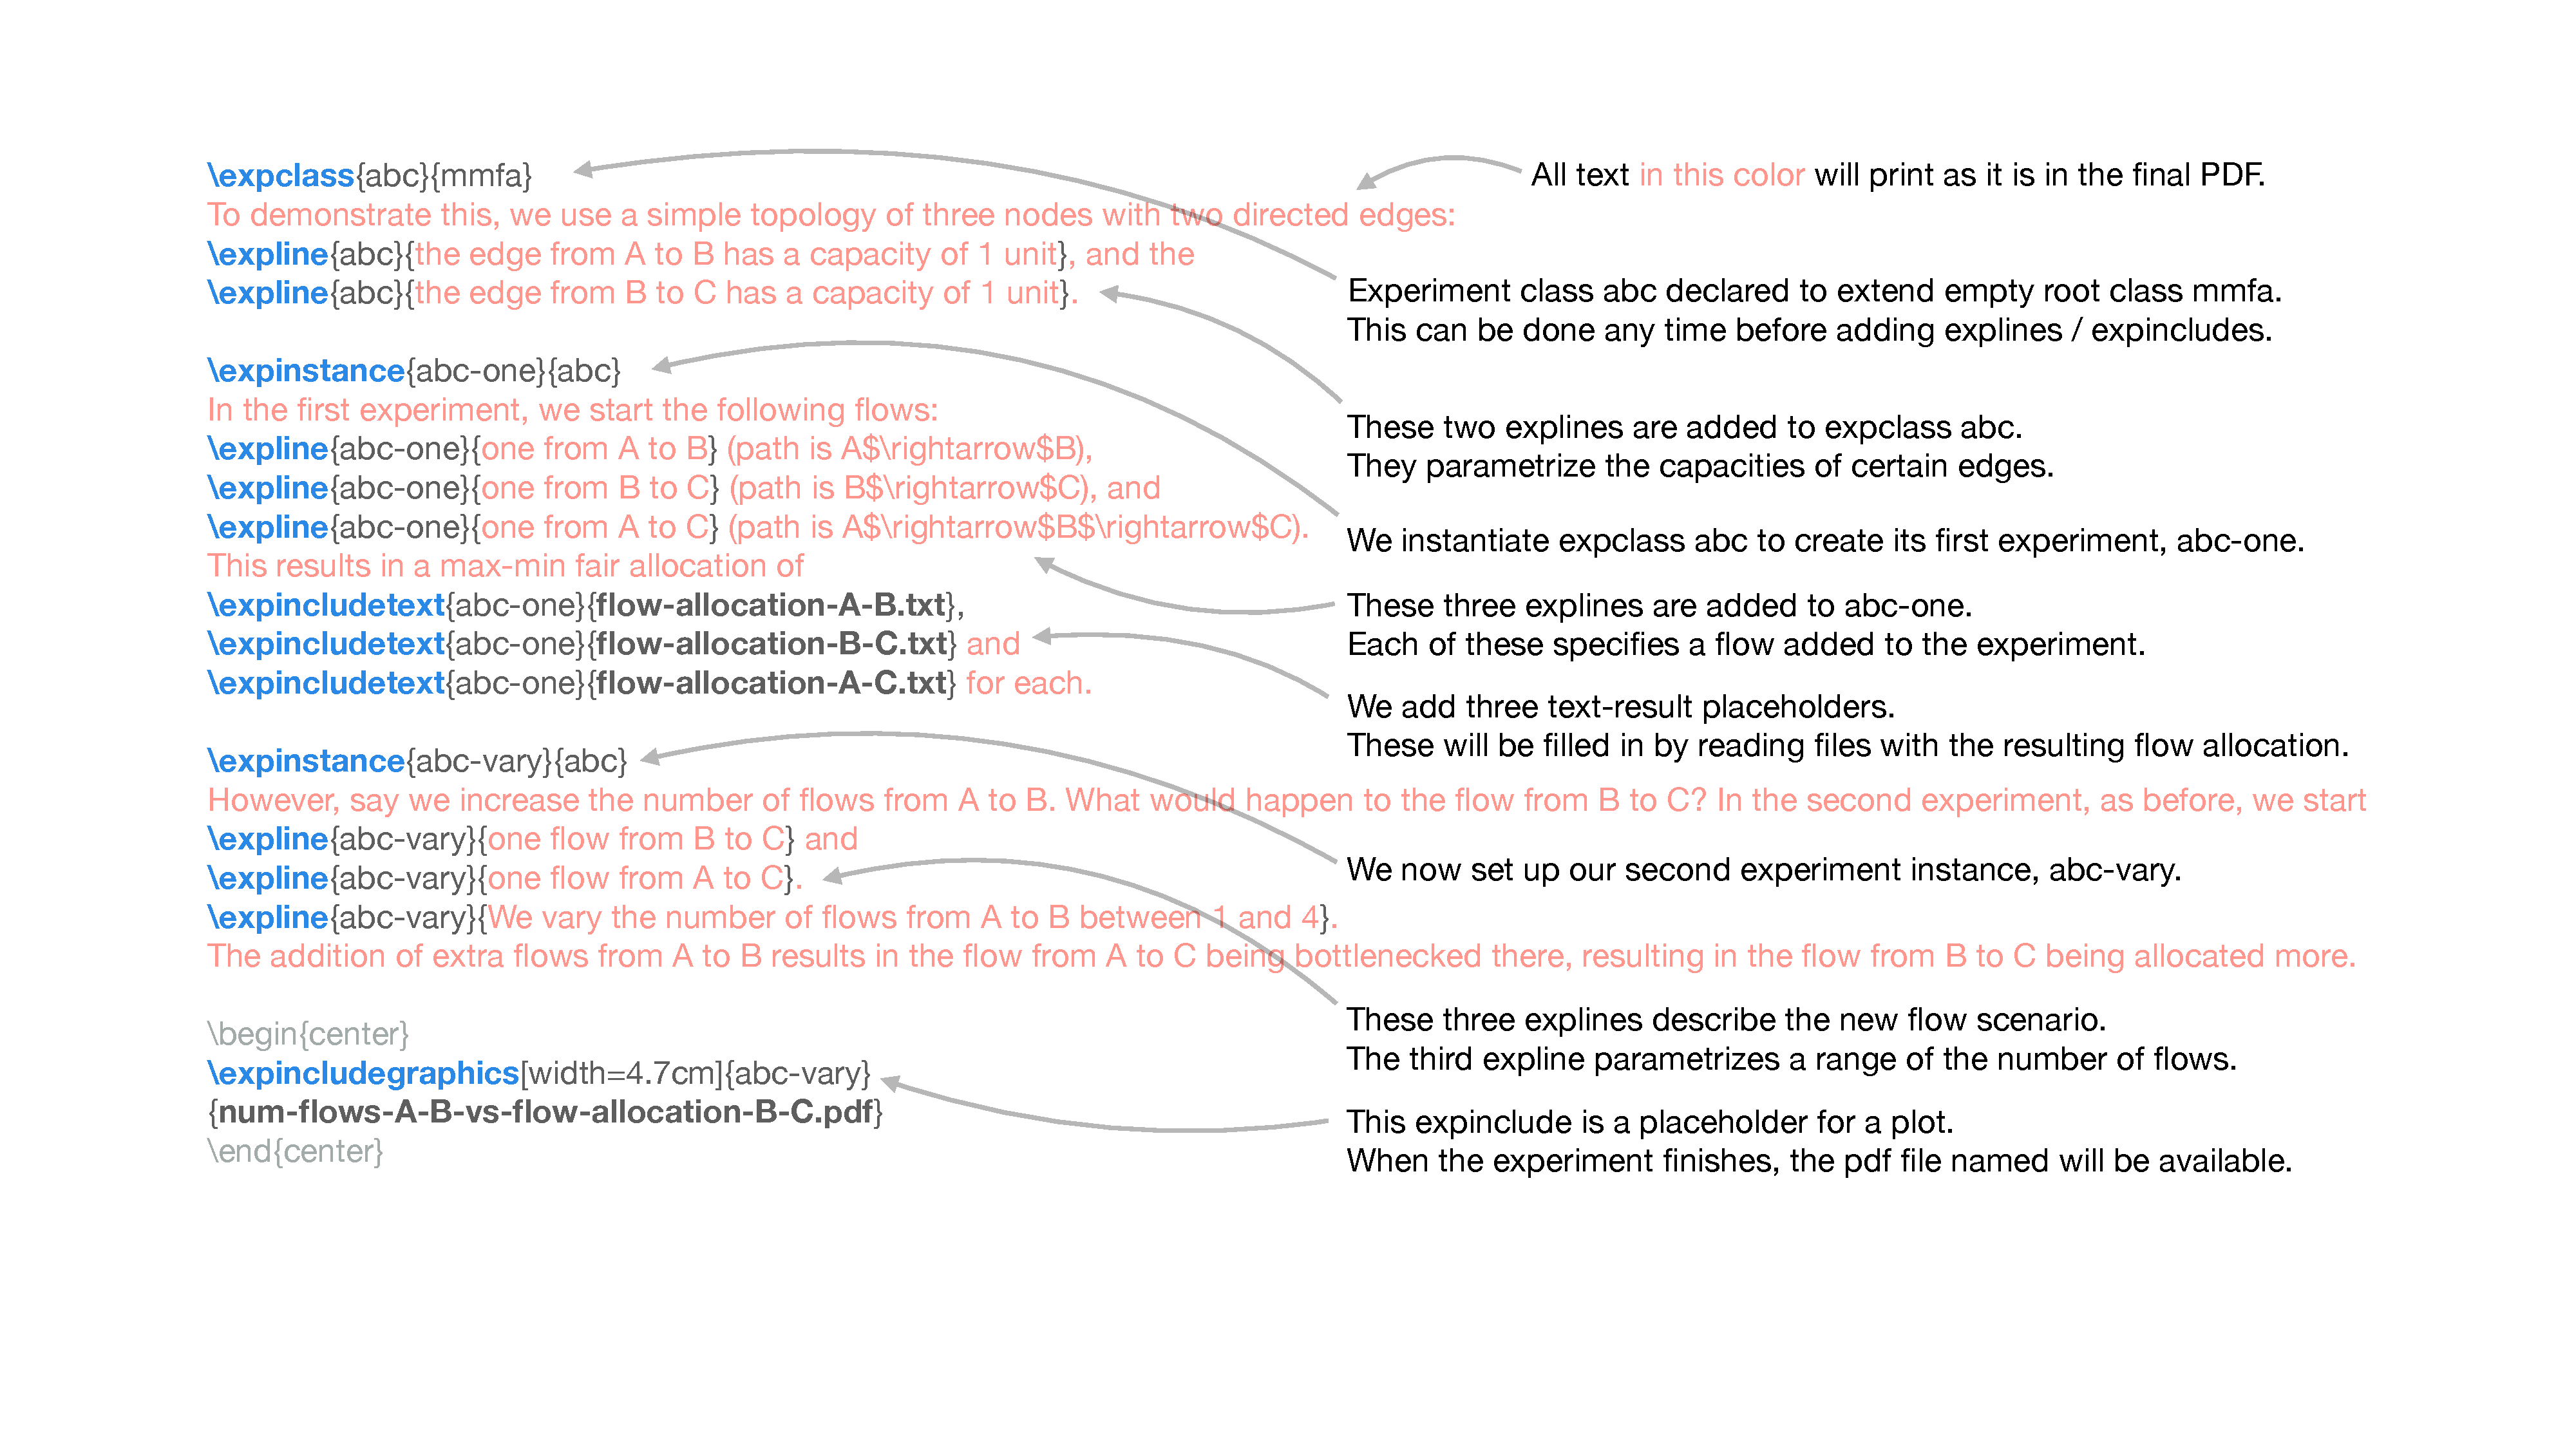
\includegraphics[width=\textwidth]{figures/markup-example.pdf}
    \caption{\LaTeX{} source for the max-min fairness example. There are two experiment instances \texttt{abc-one} and \texttt{abc-vary}, both of which inherit from class \texttt{abc}. The flow scenarios are described for each using \texttt{explines}. For the first experiment, three text results, one value for each of the three flow allocations, will be read from the files specified after the experiment runs. For the second one, the plot in the file specified using \texttt{expincludegraphics} will be inserted.}
    \label{fig:example-latex}
    \vspace{-6pt}
\end{figure*}

\noindent All of the above markup is used internally by our \experimentex parser (and subsequently, author-defined interpretations of it), but only the \textbf{bold} parts have direct, visible impact on the final PDF document compiled by \LaTeX{}. The explines are printed as is --- this is key to ensuring consistency between what is written and what is run in the experiments. The two types of expincludes behave like the \texttt{\textbackslash{}input} and \texttt{\textbackslash{}includegraphics} \LaTeX{} commands, and are used to add result text and result plots respectively.

Fig.~\ref{fig:example-latex} shows the \LaTeX{} code for the max-min fairness example from \S\ref{sec:example}. Some superfluous parts, like the opening preamble text and the topology graphic, are excluded for brevity.

By default, all \experimentex commands are ``safe'' in that they do not cause warnings or errors if the \LaTeX{} source is compiled without running the experiments via \sysname. In this case, the placeholders for experiment results simply show default text and figure placeholders --- Appendix~\ref{sec:compile-like-normal} shows what this looks like for the max-min fairness text. The grammatical validity, \eg inheritance and naming, is only appraised when the \experimentex parser runs (\S\ref{sec:parser}). Whether the explines translate to valid runs is only determined once the interpreter runs over the parser's output (\S\ref{sec:interpreter}). The validity of the output results is only determined once the plotter has run over the parser's output representation, combined with the runs' output log files (\S\ref{sec:plotter}).

%%%%%%%%%%%%%%%%%%%%%%%%%%%%%%%%%%%%%%%%%%%%%%%%%%%%%%
%%%%%%%%%%%%%%%%%%%%%%%%%%%%%%%%%%%%%%%%%%%%%%%%%%%%%%
%%%%%%%%%%%%%%%%%%%%%%%%%%%%%%%%%%%%%%%%%%%%%%%%%%%%%%
%%%%%%%%%%%%%%%%%%%%%%%%%%%%%%%%%%%%%%%%%%%%%%%%%%%%%%
%%%%%%%%%%%%%%%%%%%%%%%%%%%%%%%%%%%%%%%%%%%%%%%%%%%%%%

\subsection{Parsing \experimentex}
\label{sec:parser}

The parser uses the TexSoup package~\cite{texsoup} for the initial TeX parsing, but only targets the found \experimentex commands in the \LaTeX{} source. The authors supply the parser with a list of root experiment class names. For each root class, the parser outputs a tree, whose directed edges represent the inheritance between experiment instances and classes, which are its nodes. Every node has a list of explines. Only the leaves, \ie experiment instances, additionally have a list of expincludes. The interpreter uses the parsed tree to create and performs runs, and the plotter uses it to (after the runs) know which outputs to generate. The parser guarantees that the tree satisfies various constraints, \eg names must be declared first and must be unique; after extending a class, it cannot have more explines declared; and instances cannot be extended from.

In our running example, there is only one root class, \texttt{mmfa}, so only one tree is output by the parser, shown in Fig.~\ref{fig:parsed-tree}.

The parser creates the tree, but does not check whether the explines are valid, which is the interpreter's task (see \S\ref{sec:interpreter}), nor does it check whether the expinclude filenames are valid, which is the plotter's task (see \S\ref{sec:plotter}). As such, the parser is the same for all \sysname papers, and does not need to be edited by the authors.

\begin{figure}
    \centering
    % Source file: figures/parsed-tree.key
    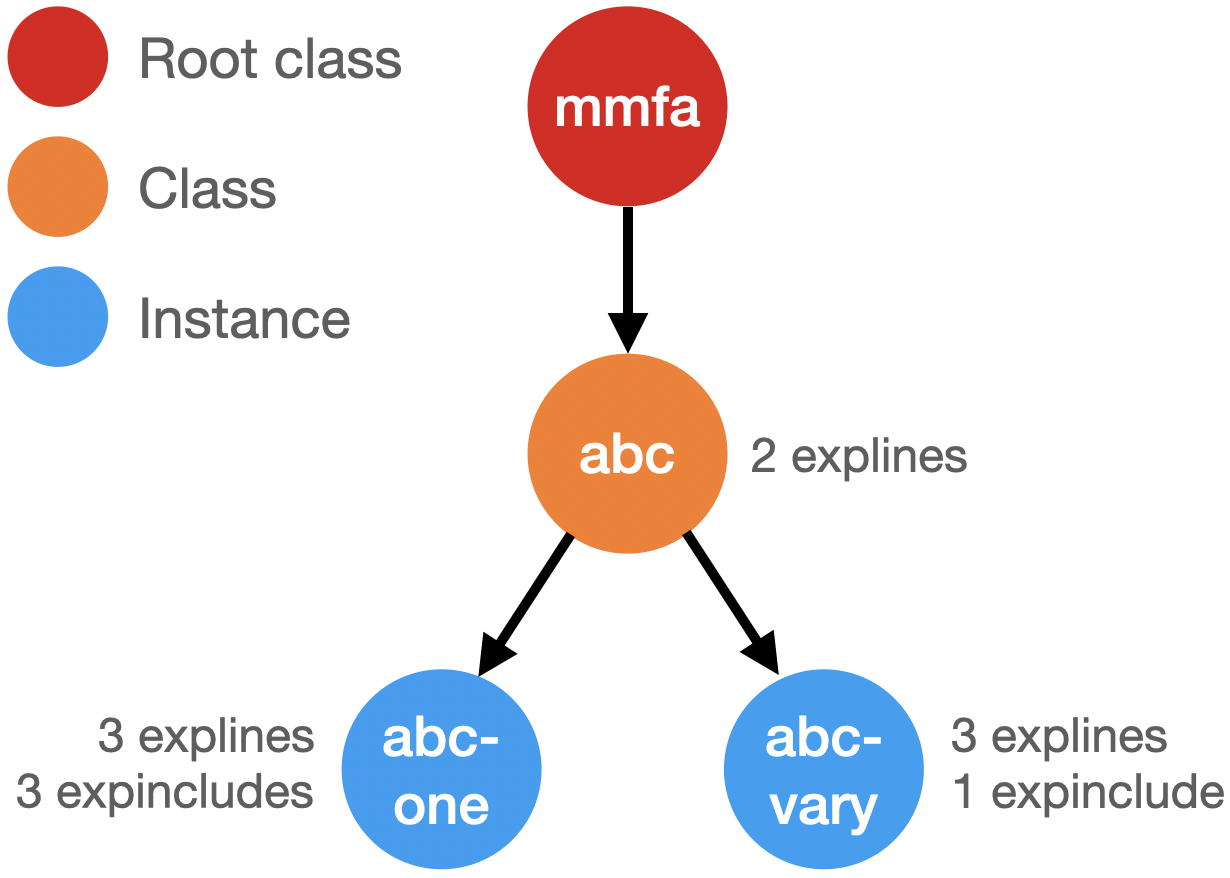
\includegraphics[width=0.3\textwidth]{figures/parsed-tree.png}
    \caption{Parsed tree for the max-min fairness example of \S\ref{sec:example}.}
    \label{fig:parsed-tree}
    \vspace{-14pt}
\end{figure}

%%%%%%%%%%%%%%%%%%%%%%%%%%%%%%%%%%%%%%%%%%%%%%%%%%%%%%
%%%%%%%%%%%%%%%%%%%%%%%%%%%%%%%%%%%%%%%%%%%%%%%%%%%%%%
%%%%%%%%%%%%%%%%%%%%%%%%%%%%%%%%%%%%%%%%%%%%%%%%%%%%%%
%%%%%%%%%%%%%%%%%%%%%%%%%%%%%%%%%%%%%%%%%%%%%%%%%%%%%%
%%%%%%%%%%%%%%%%%%%%%%%%%%%%%%%%%%%%%%%%%%%%%%%%%%%%%%

\subsection{Interpreter: invoking experiments}
\label{sec:interpreter}

For each root experiment class, $r$, the authors write an interpreter. The interpreter takes $r$'s parsed tree, and translates it into experiment runs that can be executed by the authors' chosen frameworks. Writing an interpreter entails four tasks.

\parab{Task 1: define the root data structure}\\
The interpreter defines an empty root data structure, which contains the parameters that can be set by explines.

In our running example, we want to experiment with a (fixed) three node topology with two directed links (A$\rightarrow$B, B$\rightarrow$C). There are two parametrizable aspects: the link capacities and the flow scenario. We thus define root class \texttt{mmfa} with the following data structure:
\vspace{-0in}
\begin{verbatim}
DATA STRUCTURE mmfa {
  cap_A_B: float
  cap_B_C: float
  num_flows_A_B: integer (or list[integer])
  num_flows_B_C: integer (or list[integer])
  num_flows_A_C: integer (or list[integer])
}
\end{verbatim}
\vspace{-0in}
\noindent To allow multiple runs across a range of values for a parameter, we use lists in the data structures. In the above example, the number of flows between each pair of nodes can be varied. If each of the three flow counts uses such a range instead of one value, we end up with a Cartesian product of runs.

\parab{Task 2: interpret explines into data structures}\\
The interpreter goes through the parsed tree starting from the root, and interprets the explines defined for each node to fill in the data structure. Every child of a node receives a copy of the data structure of its parent, thus inheriting all its explines. Each leaf must end up with a fully filled-in root data structure. Only leaves, \ie experiment instances, will be converted into one or more run directories for a certain framework.

What constitutes a valid expline, its \textit{template}, must be intuitive and its effect on the underlying data structure predictable. However, the explines are sentences which will literally be displayed in the final paper: we do not want to restrict authors to being only able to form rigid flow-breaking sentences because they must match a certain format. The best of both worlds can be achieved by combining regular expression (regex) matching (deterministic, but rigid) with an iterative writing approach (\S\ref{sec:writing-strategy}). Every iteration after the authors have edited the text, they add, extend and/or update the regular expression and the parsing of their grouped values. Typically, few changes are required in the interpreter apart from the addition, removal and reordering of filler words in the regex pattern.

The explines are processed sequentially in deterministic reading order from the start to the end of the paper's LaTeX. The interpreter must evaluate explines and update the data structure accordingly. The interpreter throws an error if the expline does not match a template, if the values are incorrect, or if the expline is invalid given the current state of the data structure (\eg due to conflict with a previous expline).

For our running example, we define the following templates to be valid for our interpreter:
\vspace{-0in}
\begin{verbatim}
(1) The edge from {} to {} has a capacity of {}
(2) We vary the number of flows 
    from {} to {} between {} and {}
(3) One from {} to {}
(4) One flow from {} to {}
\end{verbatim}
\vspace{-0in}
\noindent The interpreter first performs regular expression (regex) matching to identify the groups. In the regex-matching, we make sure that it is resistant whether the first letter capitalized or if there is an ending dot, and which type of white space exists between the words. The regex groups are values which are subsequently verified. It must enforce constraints such that the data structure is modified correctly: it throws an error, for example, if the values contain invalid node identifiers, non-existent links, or negative capacities. An expline must also be consistent with the effect of explines which came before, \eg setting the capacity of a link twice is not permitted. 

For greater writing flexibility, authors can iteratively augment the set of valid templates, for instance, in the above example, it may be useful to add a template to specify the capacity of all links at once.

For our example, the interpreter receives the parsed tree of Fig.~\ref{fig:parsed-tree}. It first interprets the 2 explines for class \texttt{abc} into its data structure. Afterward, the interpreter creates two copies of the data structure for the two child classes \texttt{abc-one} and \texttt{abc-vary}, and then processes the additional explines for each of them. This results in two completely filled data structures, one for each experiment instance:
\vspace{0in}
\begin{verbatim}abc-one {
  cap_A_B: 1,
  cap_B_C: 1,
  num_flows_A_B: 1,
  num_flows_B_C: 1,
  num_flows_A_C: 1
}
abc-vary { 
  cap_A_B: 1,
  cap_B_C: 1,
  num_flows_A_B: [1, 2, 3, 4],
  num_flows_B_C: 1,
  num_flows_A_C: 1
}\end{verbatim}
\vspace{-0in}
\noindent\textbf{Task 3: translate data structures into run directories}\\
The interpreter prepares for invoking the authors' run framework(s) by creating a directory for each individual run. If an experiment instance's data structure only has attributes which are single-valued, it will directly map to a single run directory. If it has attributes which are multi-valued, it leads to a Cartesian product of single-valued data structures, and an equal number of run directories. A run directory is thus self-contained from the perspective of the run framework, providing both the inputs and a location for the outputs. The directory translation has the following components:

\begin{itemize}[leftmargin=12pt,itemsep=2pt,topsep=2pt]

    \item \textbf{Naming and look-up.} We name a run directory by appending its root class name with a hash of its data structure. Using the root class name, instead of experiment instance, eliminates duplicate runs across instances. For human readability, and correctness despite (unlikely) hash collisions (default: SHA-256), 
    we add to each run folder a file containing a full string representation of its data structure.
    
    \item \textbf{Mapping for plotter.} We save a mapping of each experiment to its corresponding set of run directories such that the plotter (\S\ref{sec:plotter}) does not need to re-interpret.

    \item \textbf{Input generation.} In each run directory, we generate the input configuration files based on the data structure. For instance, for our max-min fairness example, authors fix the topology, but allow the link capacities to be changed. Their implementation of the interpreter must output link capacities to the run directory in a format their run framework uses. After generating the input data for a run, we echo ``Yes'' to a file in its directory, \textit{input-ready.txt}.
    
\end{itemize}

\noindent In our running example, there are two data structures. \texttt{abc-one} is already single-valued. \texttt{abc-vary} is multi-valued and results in four single-valued data structures. Of the five single-valued data structures, four are unique. As such, only four run directories are created. The mapping, however, remains in place: \texttt{abc-one} maps to one run directory, and \texttt{abc-vary} maps to four run directories. An overview of the run directories is in Fig.~\ref{fig:runs}.

\begin{figure}
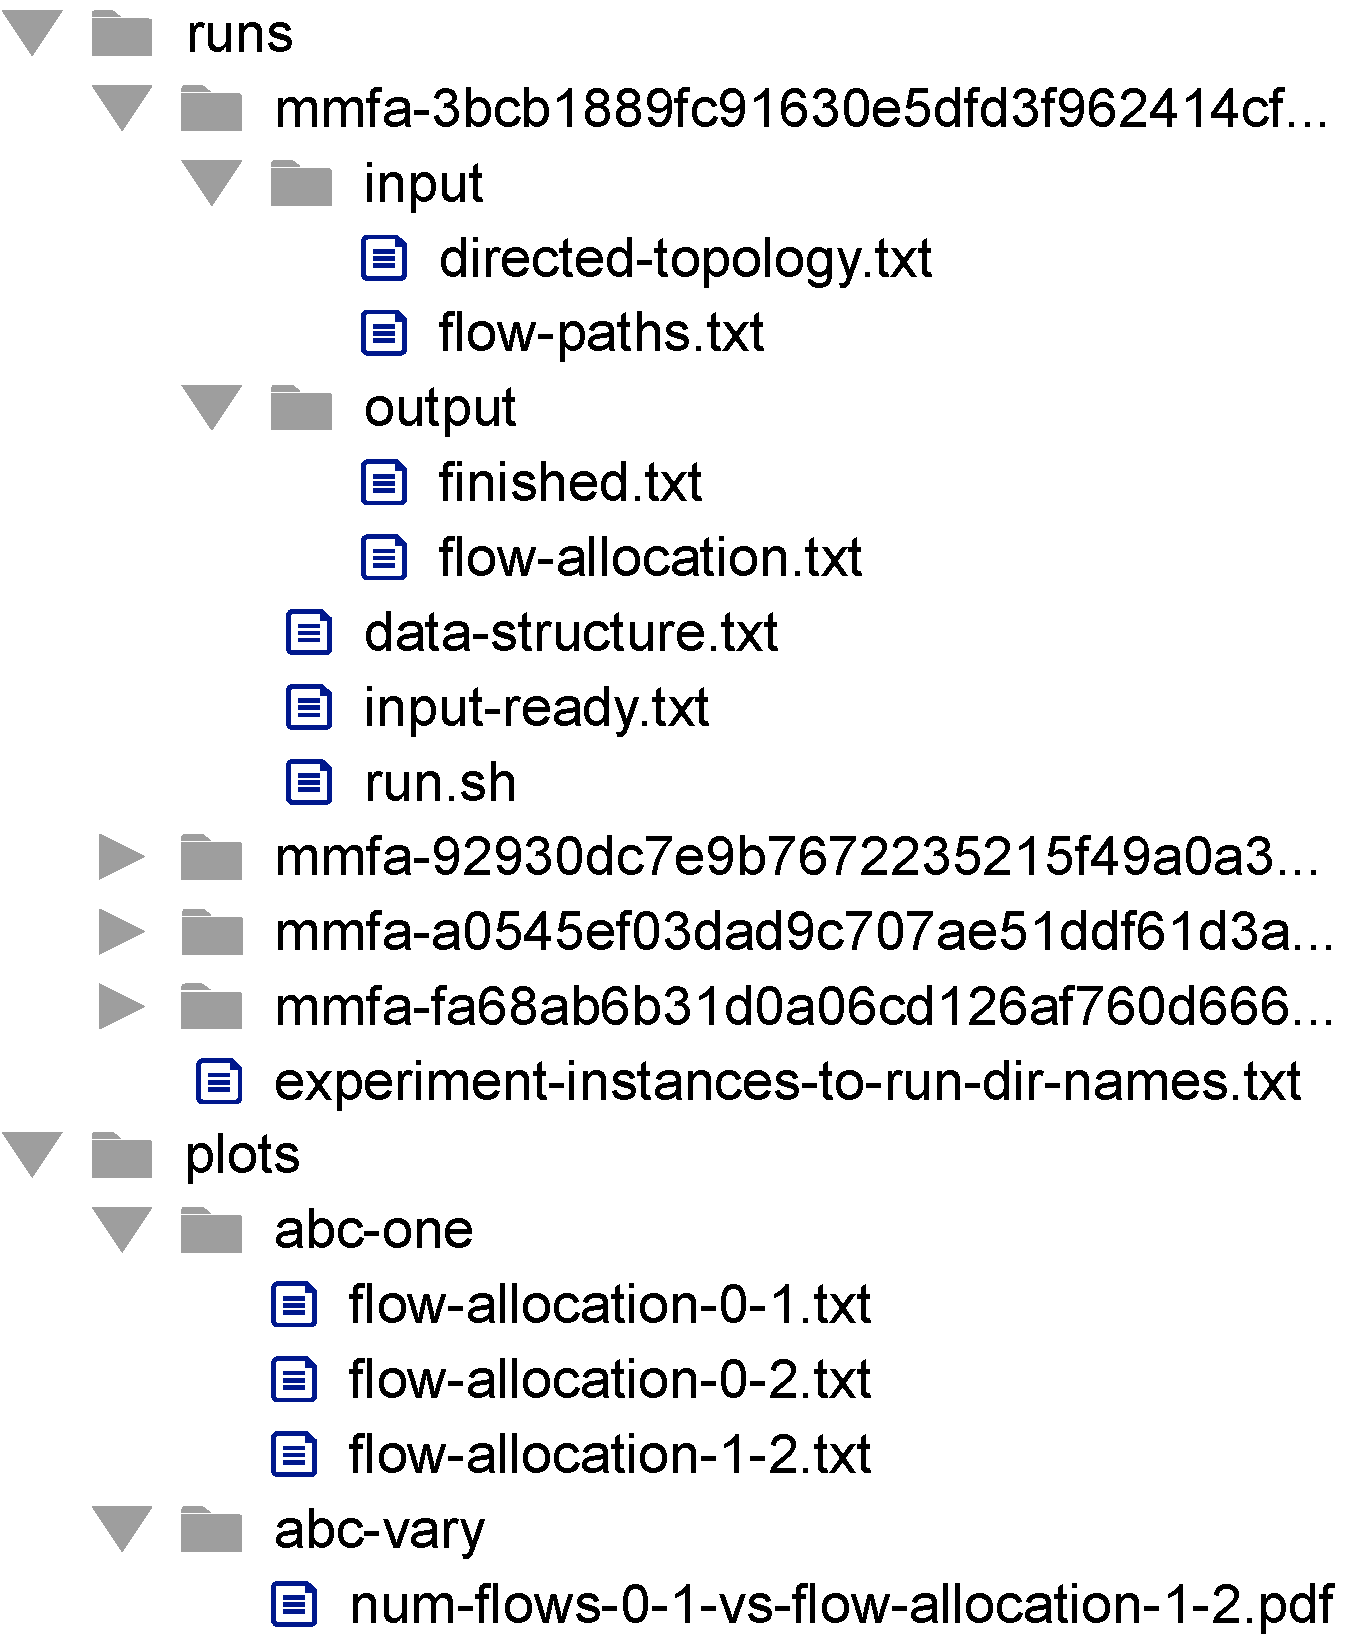
\includegraphics[width=0.35\textwidth]{figures/runs-plots.pdf}
\caption{Runs, plots folders of the max-min fairness example.}
\label{fig:runs}
\vspace{-6pt}
\end{figure}

\parab{Task 4: generate run script for each run directory}\\
As its final task, the interpreter generates a bash execution script, \textit{run.sh}, for each run folder. In its \textit{run.sh} script, it should call on its run framework to process the input, and output its logs into the run directory. After the interpret phase for all root classes finishes, our current implementation walks sequentially through the runs directory, executing each \textit{run.sh} file. Of course, this can also be done using a more sophisticated job scheduler, \eg to accommodate parallel executions.

For our max-min fairness example, running the \textit{run.sh} in a directory first checks whether the output folder already contains a \textit{finished.txt} file indicating if this run was already executed. Otherwise, it uses Python to execute a max-min fair allocation solver, the input to which are the paths to the run's input and output directories. (The implemented max-min fair allocation algorithm is based on section II.B of \cite{nace2006} and uses networkx~\cite{networkx} for graph data structures.)

%%%%%%%%%%%%%%%%%%%%%%%%%%%%%%%%%%%%%%%%%%%%%%%%%%%%%%
%%%%%%%%%%%%%%%%%%%%%%%%%%%%%%%%%%%%%%%%%%%%%%%%%%%%%%
%%%%%%%%%%%%%%%%%%%%%%%%%%%%%%%%%%%%%%%%%%%%%%%%%%%%%%
%%%%%%%%%%%%%%%%%%%%%%%%%%%%%%%%%%%%%%%%%%%%%%%%%%%%%%
%%%%%%%%%%%%%%%%%%%%%%%%%%%%%%%%%%%%%%%%%%%%%%%%%%%%%%

\subsection{Plotter: consume logs, produce results}
\label{sec:plotter}

For each root class, authors build a post-processing pipeline. 

\begin{itemize}[leftmargin=12pt,itemsep=2pt,topsep=2pt]
    \item From the parser, the plotter learns which plot files to generate for each experiment instance, as declared through \texttt{\textbackslash expincludetext} and \texttt{\textbackslash expincludegraphics}.
    
    \item From the interpreter it learns which run directories exist for each experiment instance by reading \textit{experiment-instances-to-run-dir-names.txt}.
    
    \item For each experiment instance, it creates a directory in the \textit{plots} directory in which it places the output plot files.
    
    \item For each experiment instance, it goes over the list of plot files and generates them one after the other. A plot file can use both experiment input and output data.
    
\end{itemize}

\noindent For our running example, we can generate the following files from processing the experiment results:

\begin{itemize}[leftmargin=12pt,itemsep=2pt,topsep=2pt]
    \item \textit{flow-allocation-(from)-(to).txt} : Amount allocated to each flow between the from and to nodes, without trailing zeroes. Such files are only generated for an experiment instance which maps to a single run directory.
    \item \textit{num-flows-(from)-(to)-vs-flow-allocation-(src)-(dst).pdf} : 2D plot, with the $x$-axis being the number of flows between the \textit{from} and \textit{to} nodes, and the $y$-axis being the amount of flow allocated to each flow from \textit{src} to \textit{dst}.
\end{itemize}

%%%%%%%%%%%%%%%%%%%%%%%%%%%%%%%%%%%%%%%%%%%%%%%%%%%%%%
%%%%%%%%%%%%%%%%%%%%%%%%%%%%%%%%%%%%%%%%%%%%%%%%%%%%%%
%%%%%%%%%%%%%%%%%%%%%%%%%%%%%%%%%%%%%%%%%%%%%%%%%%%%%%
%%%%%%%%%%%%%%%%%%%%%%%%%%%%%%%%%%%%%%%%%%%%%%%%%%%%%%
%%%%%%%%%%%%%%%%%%%%%%%%%%%%%%%%%%%%%%%%%%%%%%%%%%%%%%

\subsection{Final product: PDF generation}

After all the promised output plot files have been generated, the \texttt{\textbackslash expincludetext} and \texttt{\textbackslash expincludegraphics} commands will include the promised resources into the paper correctly. A standard \LaTeX{} compilation pipeline with, \eg pdflatex and bibtex, suffices to generate the paper. To this end, we make use of TeX Live~\cite{texlive}.
